%!TEX root = ../dissertation.tex
%\begin{savequote}[75mm]
%This is some random quote to start off the chapter.
%\qauthor{Firstname lastname}
%\end{savequote}

\chapter{Dataset}

In this chapter it will be presented the dataset that has been utilized for this work. As previously mentioned, the main focus is asked to be italian automotive forums, so the first phase consisted in the search of reliable resources from which retrieve the needed information. Information retrieval has been made by crawling the founded web forums. After getting all the information, the final phase for what concerns the dataset consists on annotate all the forums' comments on the base of diverse topics. \\
In the following sections the whole procedure has been presented in detail.

\section{Dataset Retrieval}

Sentiment analysis is a practical natural language processing problem, most commonly faced involving machine learning techniques. As discussed in detail in Chapter 2, machine learning algorithms need a set of labeled data that represent the environment where the algorithm is supposed to work on. As good sampled data represent the true data distribution, as good the model should work on the real environment, so the dataset retrieval is fundamental for the final outcomes.\\
This work is focused on italian automotive forums, so the first important phase is to identify some reliable resources where to extrapolate the needed information. 


\subsection{Forums' List}

Web forums are websites (or sections of websites) that allow visitors to communicate with each other by posting messages. Most forums allow anonymously visitors to view forum contents, except for registration-required ones. Forums are available for all kinds of topics, from software to health, and like in this case, automotive. Forums are composed by user-generated content, so they are full of users' opinions then, as just mentioned, they are good environments to acquire datasets for sentiment analysis. Forums are commonly subdivided in "areas" or "rooms" which are thematic macro partitions. Rooms are again subdivided into "sections", which are discussions' categories belonging to the same thematic area. Finally, sections contain numerous "threads", which are the actual discussions.\\



For this work, target resources are identified in italian automotive web forums or blogs with possibility of discussion, with an active community. The identified resources are: Quattroruote(\url{https://forum.quattroruote.it/}), Autopareri (\url{https://www.autopareri.com/forum}), Bmwpassion (\url{https://www.bmwpassion.com/forum/}), Porschemania (\url{http://www.porschemania.it/discus/}) and HDmotori (\url{http://www.hdmotori.it/}). 
Some statistics are summarized in Table \ref{table:forum-list}.

\begin{table}[ht]
	\renewcommand{\arraystretch}{2.5}
	\centering
	\begin{tabular}{| >{\centering\bfseries}m{3cm} | >{\centering}m{1in} | >{\centering}m{1in} | >{\centering}m{1in} | >{\centering\arraybackslash}m{1in} | } 
		\hline
		\textbf{Resource} & \textbf{Type} & \textbf{\# Threads} & \textbf{\# Messages} & \textbf{\# Users} \\ [.2cm]
		\midrule
		Quattroruote & Forum & 121.366 & 2.413.452 & 70.707 \\ [.2cm]
		\hline
		Autopareri & Forum & n.a & 2.146.532 & 34.963 \\ [.2cm]
		\hline
		Bmwpassion & Forum & 349.259 & 7.909.297 & 78.608
		 \\ [.2cm]
		\hline
		Porschemania & Forum & n.a & n.a & n.a \\ [.2cm]
		\hline
		HDmotori & Blog & n.a. & n.a. & n.a. \\ [.2cm]
		\hline
	\end{tabular}
	\caption{Forums' statistics updated in date 15/08/2019.}
	\label{table:forum-list}
\end{table}

% TODO eventualmente spiegare qualcosa di tutti i forum

All resources except for Porschemania are brand independent, which means that are treated discussions about every automotive brands independently, while the last one is focused on Porsche \footnote{Porsche is a German sports car manufacturer located in Zuffenhausen in Stuttgart, founded in 1931 by Ferdinand Porsche.} discussions.\\
The dataset will be composed as a list of comments, so the idea is to download as mush information as possible, that is common to each resource, in order to represent precisely the environment in a structured way like a Comma Separated Values (CSV) file.

\subsection{Comments' Information}

Forums can be seen as a temporal ordered list of comments grouped into discussion. In this way the core part of representing discussions passes through the comment representation. Actually, it is irrelevant the way on which represent the information, but it is fundamental decide what information to keep. An idea is to keep all possible information common to comments of all resources, in order to even all entries in a standard way. In Figures \ref{fig:screen-quattroruote} \ref{fig:screen-autopareri} \ref{fig:screen-porschemania} \ref{fig:screen-bmwpassion} \ref{fig:screen-hdmotori} are shown one comment for each of the selected resources, with highlighted the information that have been decided to be extracted.

\begin{figure}[!hb]
	\centering
	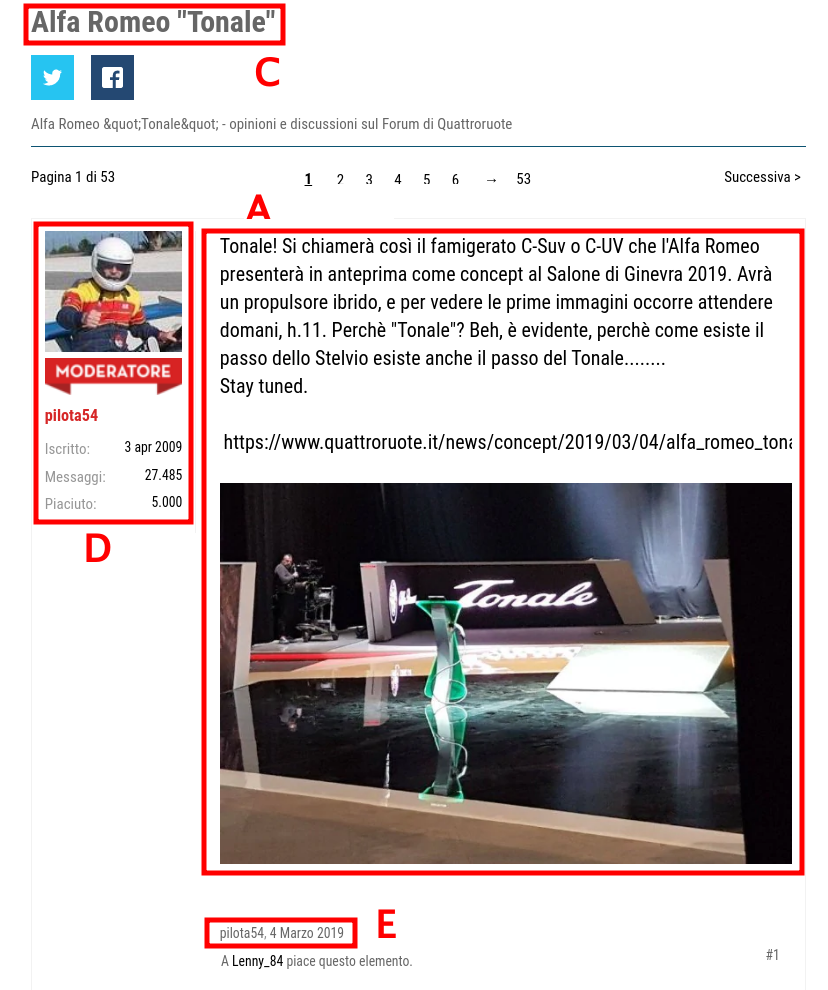
\includegraphics[width=1\textwidth]{figures/screen/screen-quattroruote.png}
	\caption{Sample comment in Quattroruote's forum}
	\label{fig:screen-quattroruote}
\end{figure}

\begin{figure}[!htb]
	\centering
	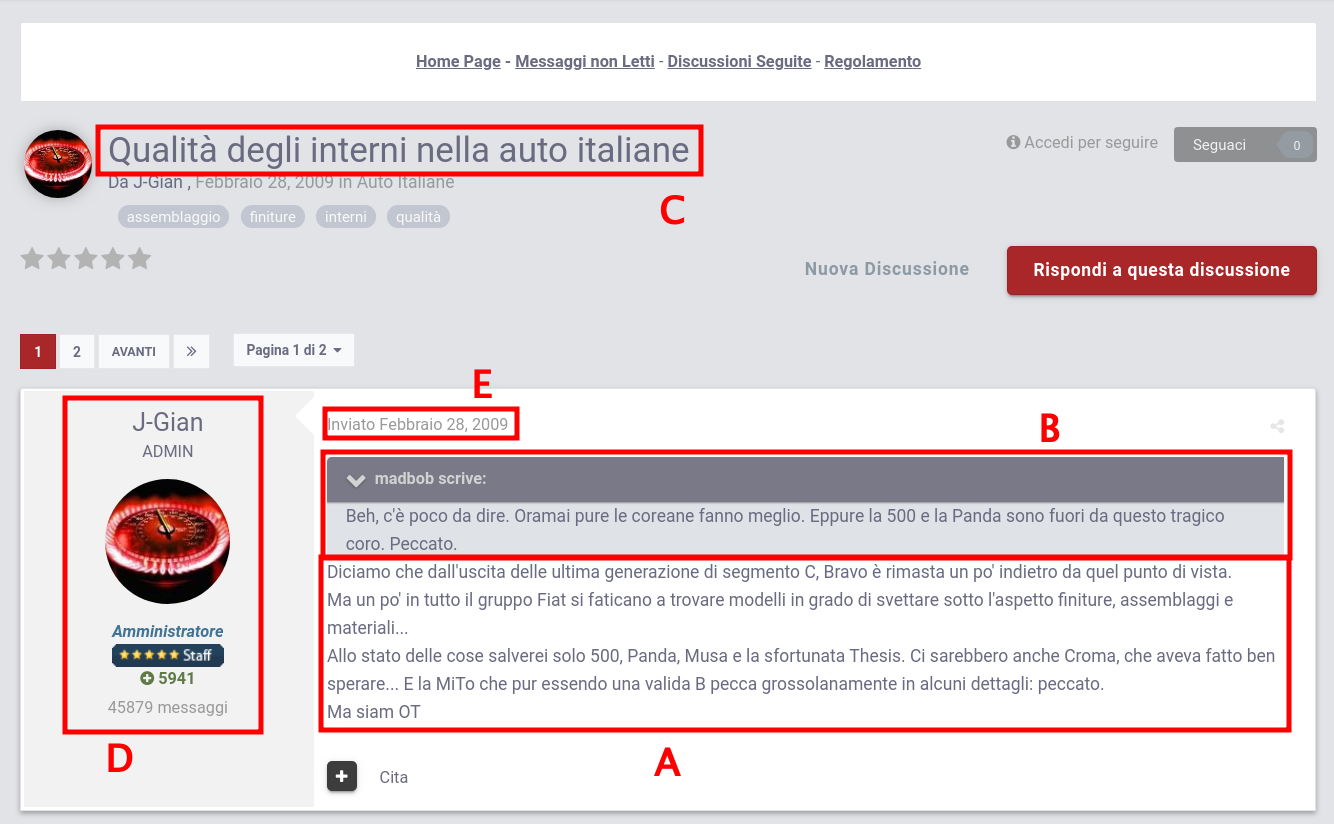
\includegraphics[width=1\textwidth]{figures/screen/screen-autopareri.png}
	\caption{Sample comment in Autopareri's forum}
	\label{fig:screen-autopareri}
\end{figure}

\begin{figure}[!htb]
	\centering
	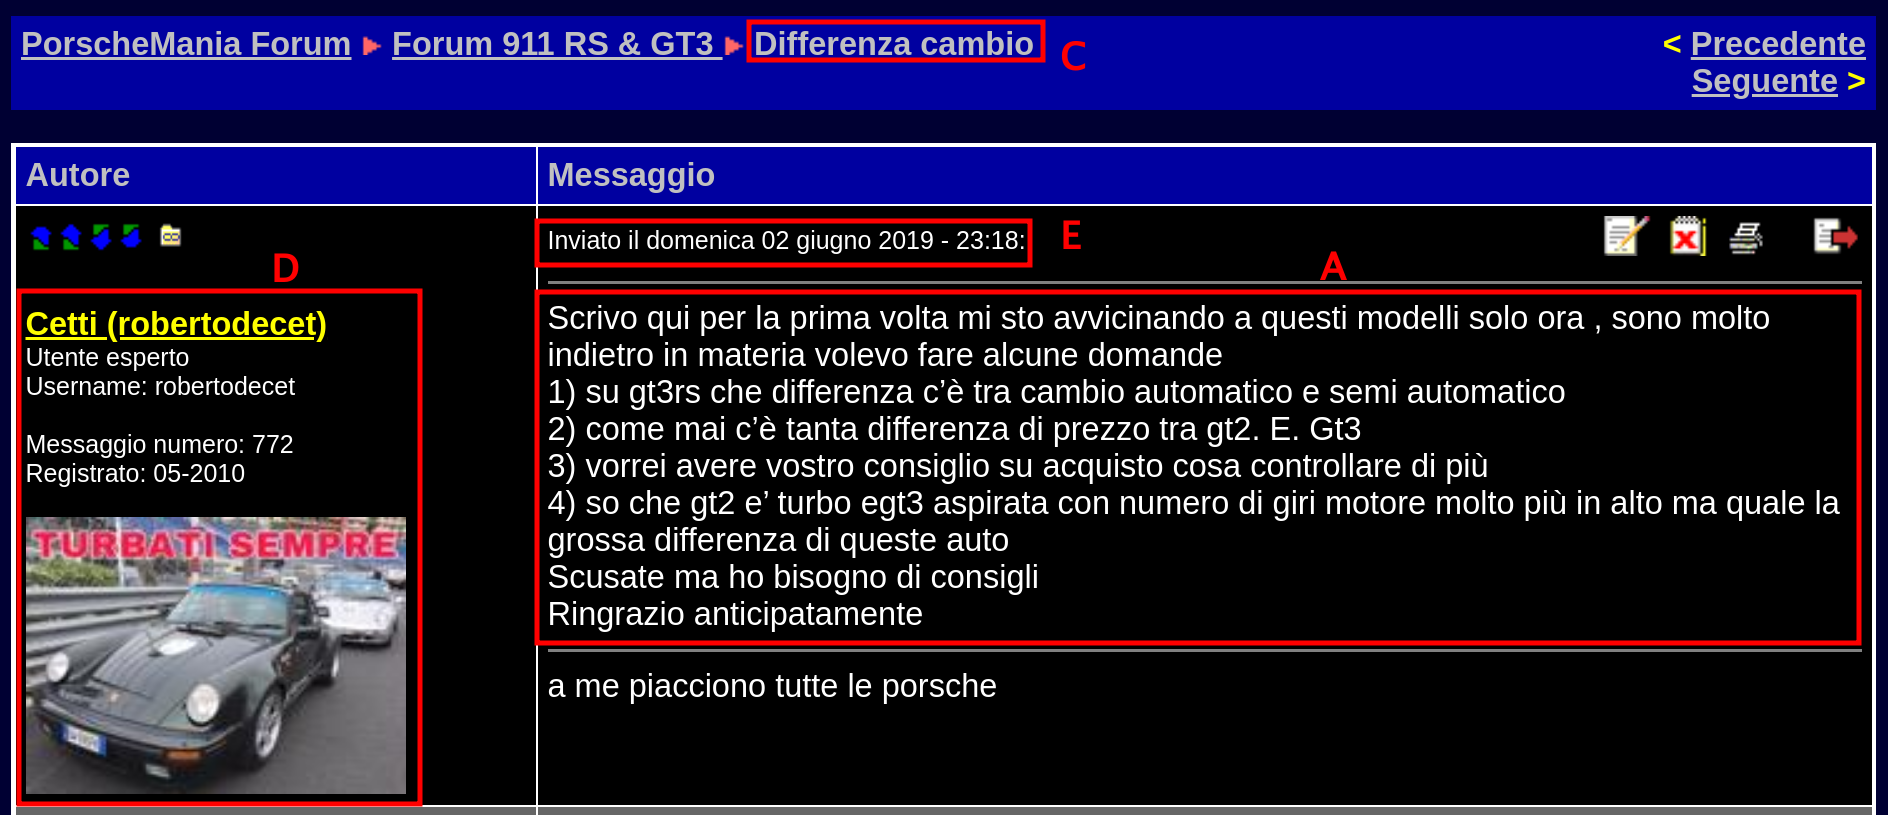
\includegraphics[width=1\textwidth]{figures/screen/screen-porschemania.png}
	\caption{Sample comment in Porschemania's forum}
	\label{fig:screen-porschemania}
\end{figure}

\begin{figure}[!htb]
	\centering
	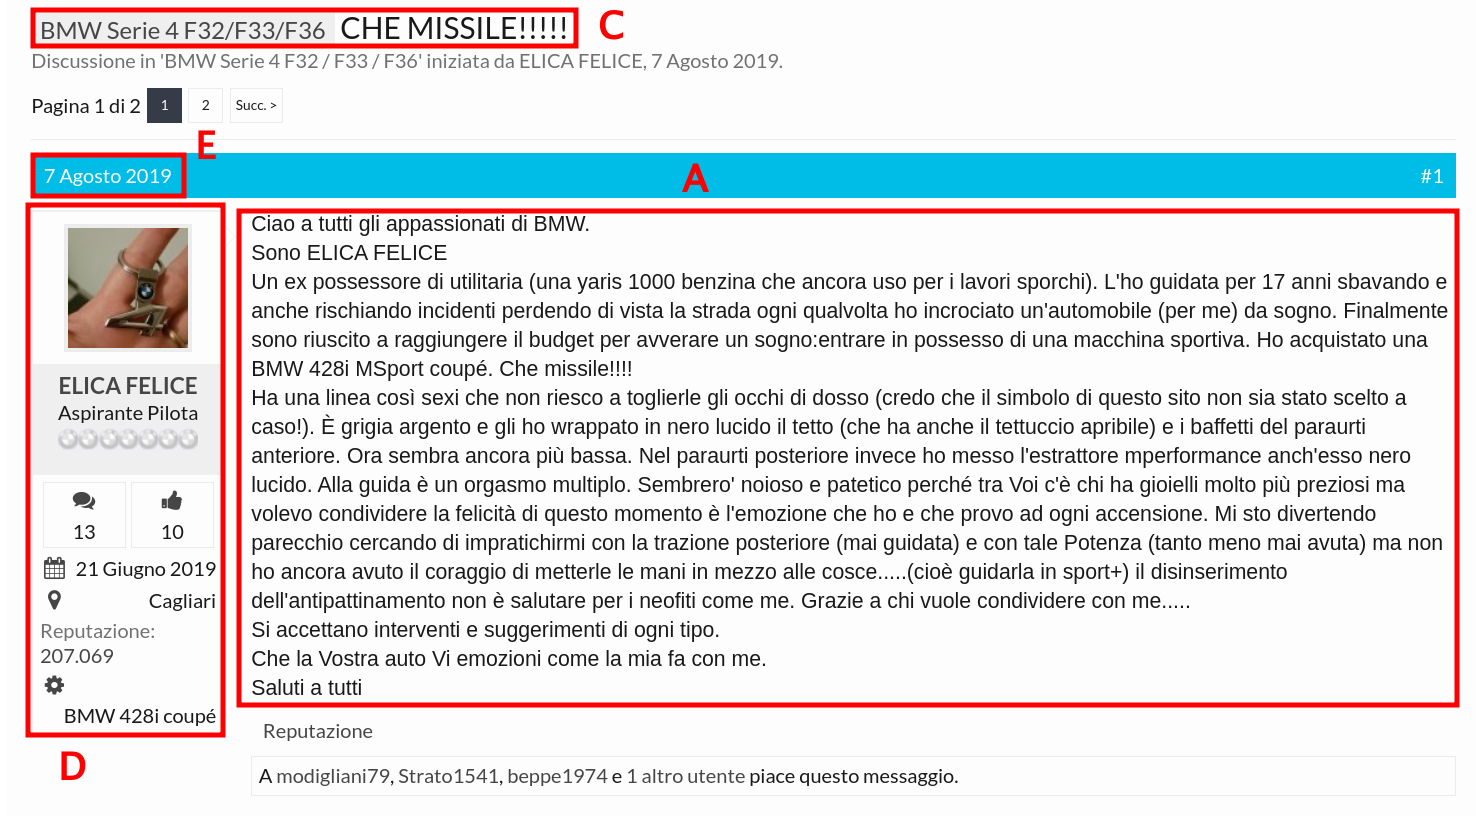
\includegraphics[width=1\textwidth]{figures/screen/screen-bmwpassion.png}
	\caption{Sample comment in Bmwpassion's forum}
	\label{fig:screen-bmwpassion}
\end{figure}

\begin{figure}[!h]
	\centering
	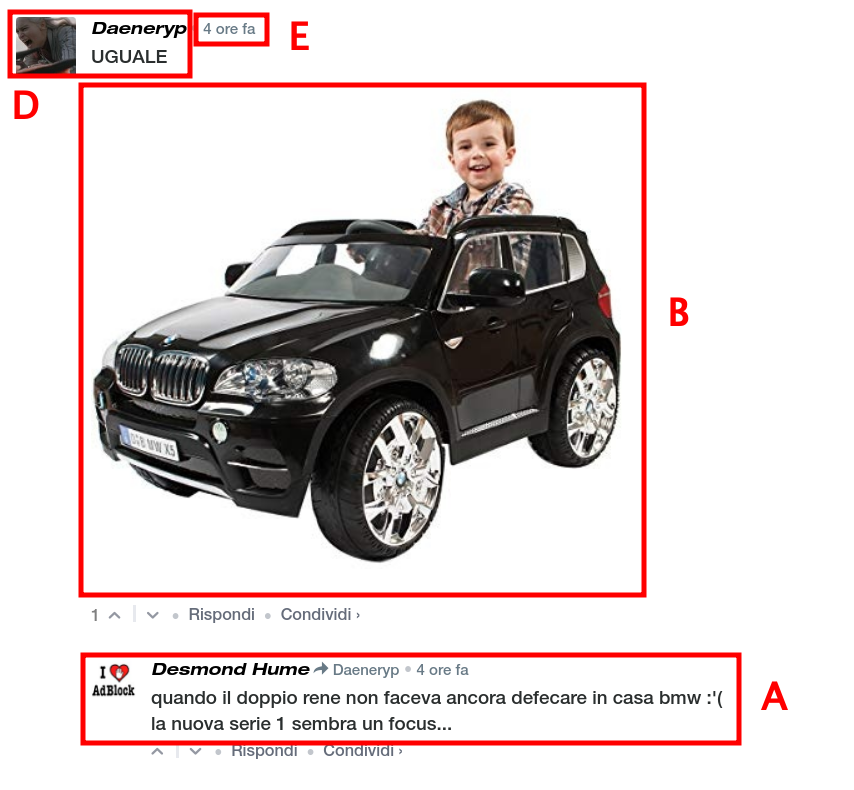
\includegraphics[width=1\textwidth]{figures/screen/screen-hdmotori.png}
	\caption{Sample comment in HDmotori's blog}
	\label{fig:screen-hdmotori}
\end{figure}

The highlighted information are summarized in the following items. The letter is the reference of the square in the image (not every item is shown because of page dimension):

\begin{itemize}
	\item \textbf{Text (A)}: the text of the comment. It is the most important information about the comment;
	
	\item \textbf{Quote (B)}: some comments may reference another user's comment in the discussion. This citation is an important information because it gives context about the text of the entry;
	
	\item \textbf{Topic's Title (C)}: the main title of the discussion;
	
	\item \textbf{Author (D)}: the username of the user that wrote the comment;
	
	\item \textbf{Comment's Timestamp (E)}: all comments contain temporal information about when they are written.
\end{itemize}


\subsection{Information Retrieval}

All information needed are viewed in web pages, but they are not accessible from any API or some other data storage interface. For this reason the only solution is to crawl all discussions' web pages and extract the information we need by parsing the HTML (Hyper-Text Markup Language) file. \\
The following paragraphs explain all information and processes used to obtain the desired data explained earlier.

\subsubsection{HTML Structure}

Web pages are written in HTML, that is a markup language designed by Tim Berners Lee in 1993. It is the standard markup language designed to be displayed in web browsers. HTML was delivered in several version: HTML 2 comes in 1995, HTML 3 in 1997, HTML 4 in 1997 and the nowadays version HTML 5 in 2014. \\
As a markup language it is composed by textual information tagged by HTML markups. A markup consists of tags which appear inside angled brackets  like "< tag >", that give information about how text should be formatted in a browser.	Most of the HTML elements are composed by two actual tags: an opening tag <tag> and a closing tag </tag>. Each element may contain other elements and so on, making HTML structured as a tree. Although several HTML markups have been introduced, a correct HTML document must always include certain tags following the standard structure:

\begin{center}
\begin{lstlisting}
<!DOCTYPE html>
<html>
   <head>
      <title>This is a title</title>
   </head>
   <body>
      <p>Hello world!</p>
   </body>
</html>
\end{lstlisting}
\end{center}

The web page content is included into the <body> tag. \\
Some commonly used HTML tags are the followings (in alphabetical order):
\begin{itemize}
	\item <!-- -->: used to define a comment that is ignored by the browser;
	\item <!DOCTYPE html>: tells the browser what kind of document it is loaded;
	\item <a>:  used to define an anchor (or hyperlink);
	\item <article>: used to contain blog entries;
	\item <b>: used to formatting the text bold;
	\item <blockquote>: used for quoting an external source;
	\item <body>: defined the body of the HTML document;
	\item <br>: single line break;
	\item <button>: defines a button that can be clicked;
	\item <caption>: used to define the table's caption;
	\item <div>: defines a container;
	\item <dl>: description list, items into <dd> or <dl> tags;
	\item <form>: forms for user inputs;
	\item <h1>, <h2>, ... , <h6>: defines headings. Lower is the number, higher is the level of the heading;
	\item <head>:  head section of the document, used for metadata;
	\item <header>: contains content to be displayed on top of the body;
	\item <html>: the root of the document. All tags must be inside this tag;
	\item <img>: displays an image;
	\item <input>: used to create forms input elements;
	\item <ol>: ordered list, items in to <li>;
	\item <style>: used for declaring inline style;
	\item <ul>: unordered list, items into <li>.
\end{itemize}

Clearly, an HTML document is a composition of all these (and other) tags, that when put together, create into the web browser a readable webpage that displays some content. Moreover, all (or almost all) HTML tags can have attributes that provide additional information about elements, specifying those in the format attribute="value" inside the start tag. This is used, for instance, in <a> tag to specify the hyperlink reference, such as:
\begin{lstlisting}
<a href="https://www.unipd.it">This is a link</a>
\end{lstlisting}
Important attributes are  "id" and "class". The value of the attribute "id"  must be unique on the entire document, while more elements can have the same value of the attribute "class". These attributes are used as selectors, for instance for defining the style or the behavior, but since it is not relevant for what concerns the information retrieval strategy, it will be not covered in detail.

\subsubsection{HTML Parser}




\subsubsection{Crawler}

Crawling is the process of automatically browsing the World Wide Web (or an interested part of it) using some programmed scripts called \textit{crawlers}.








\section{Dataset Annotation}

\section{Statistics}

